\xsection{myblue}{Categories}

\begin{frame}{Category building example: cc}
  \begin{columns}[c, onlytextwidth]
  \begin{column}{0.45\textwidth}
  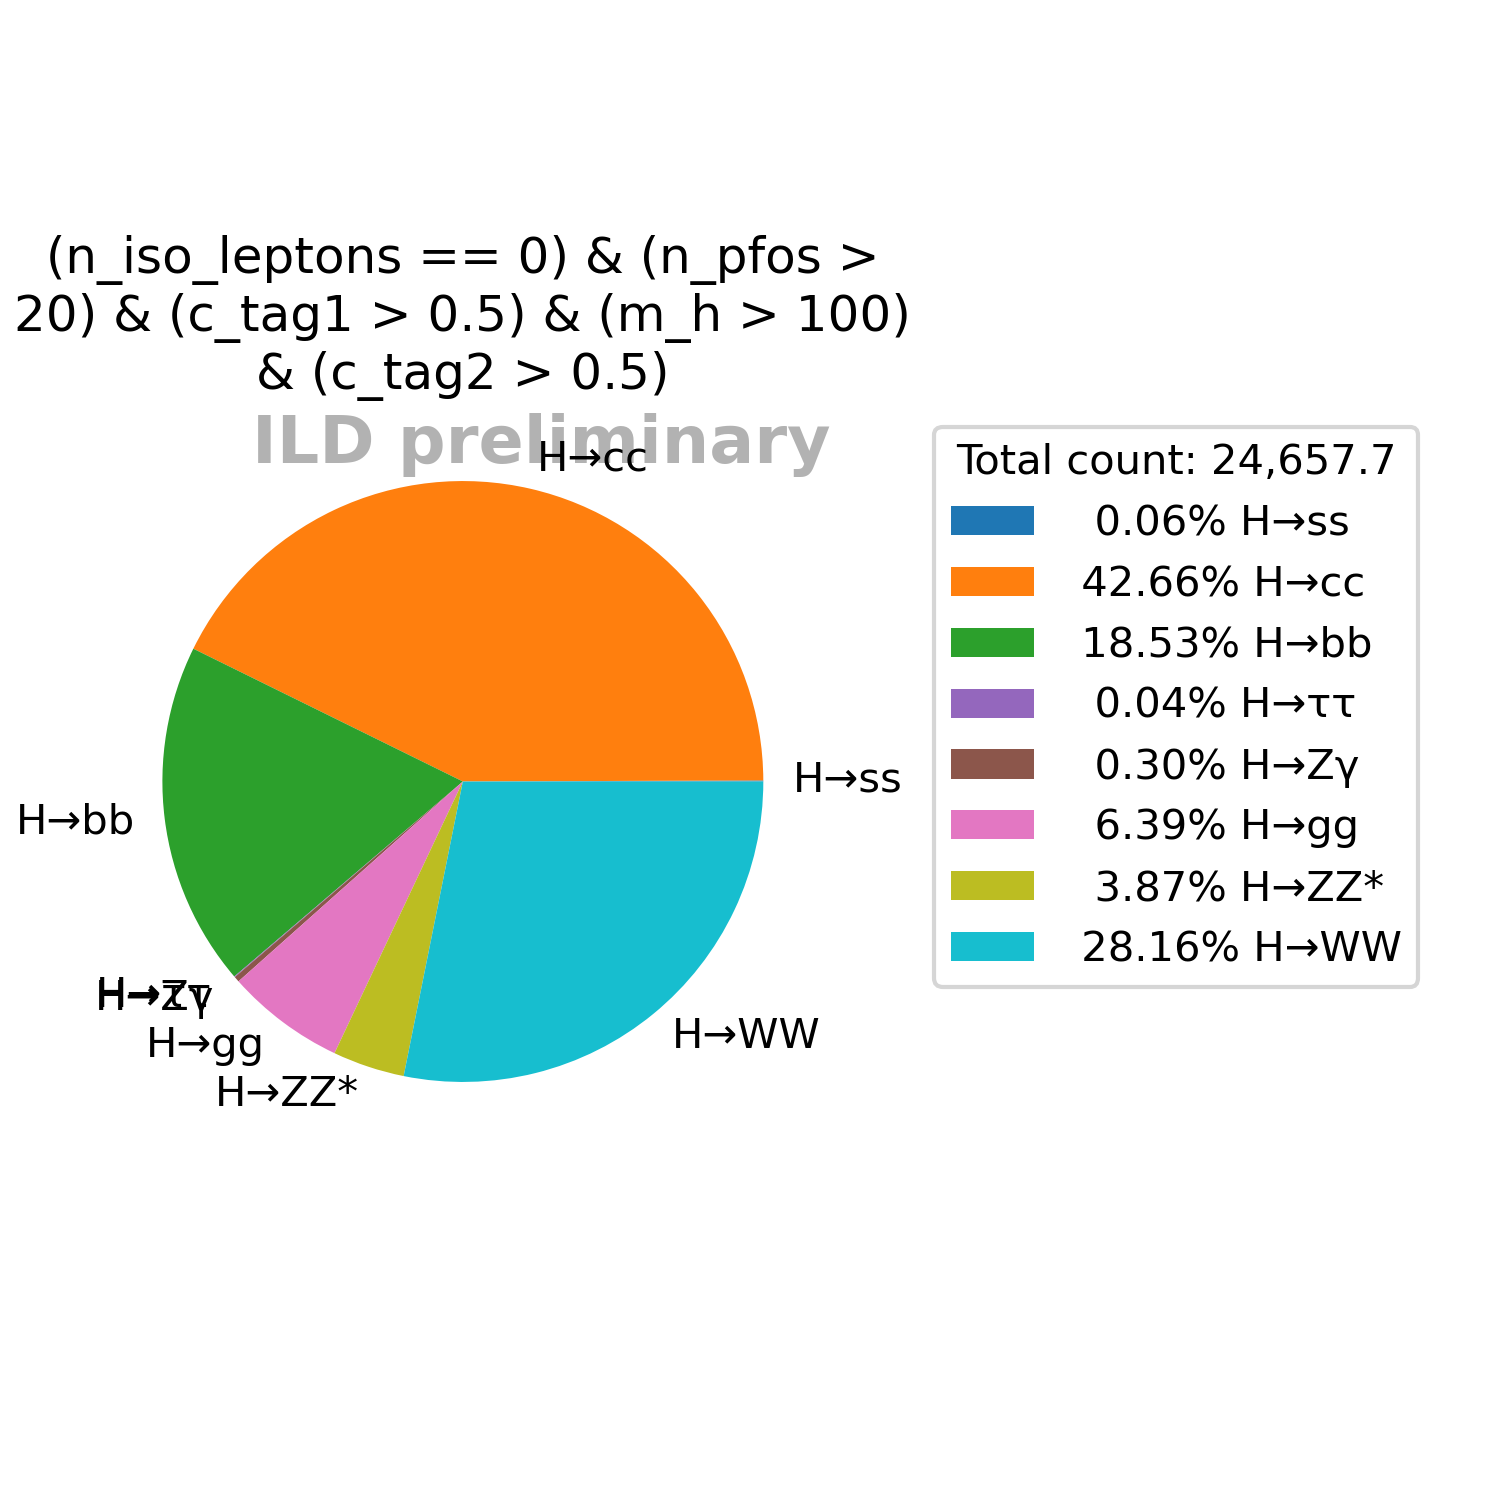
\includegraphics[width=\textwidth, keepaspectratio]
      {plot_factory/cc_category_pie}

  \end{column}
  \begin{column}{0.55\textwidth}
  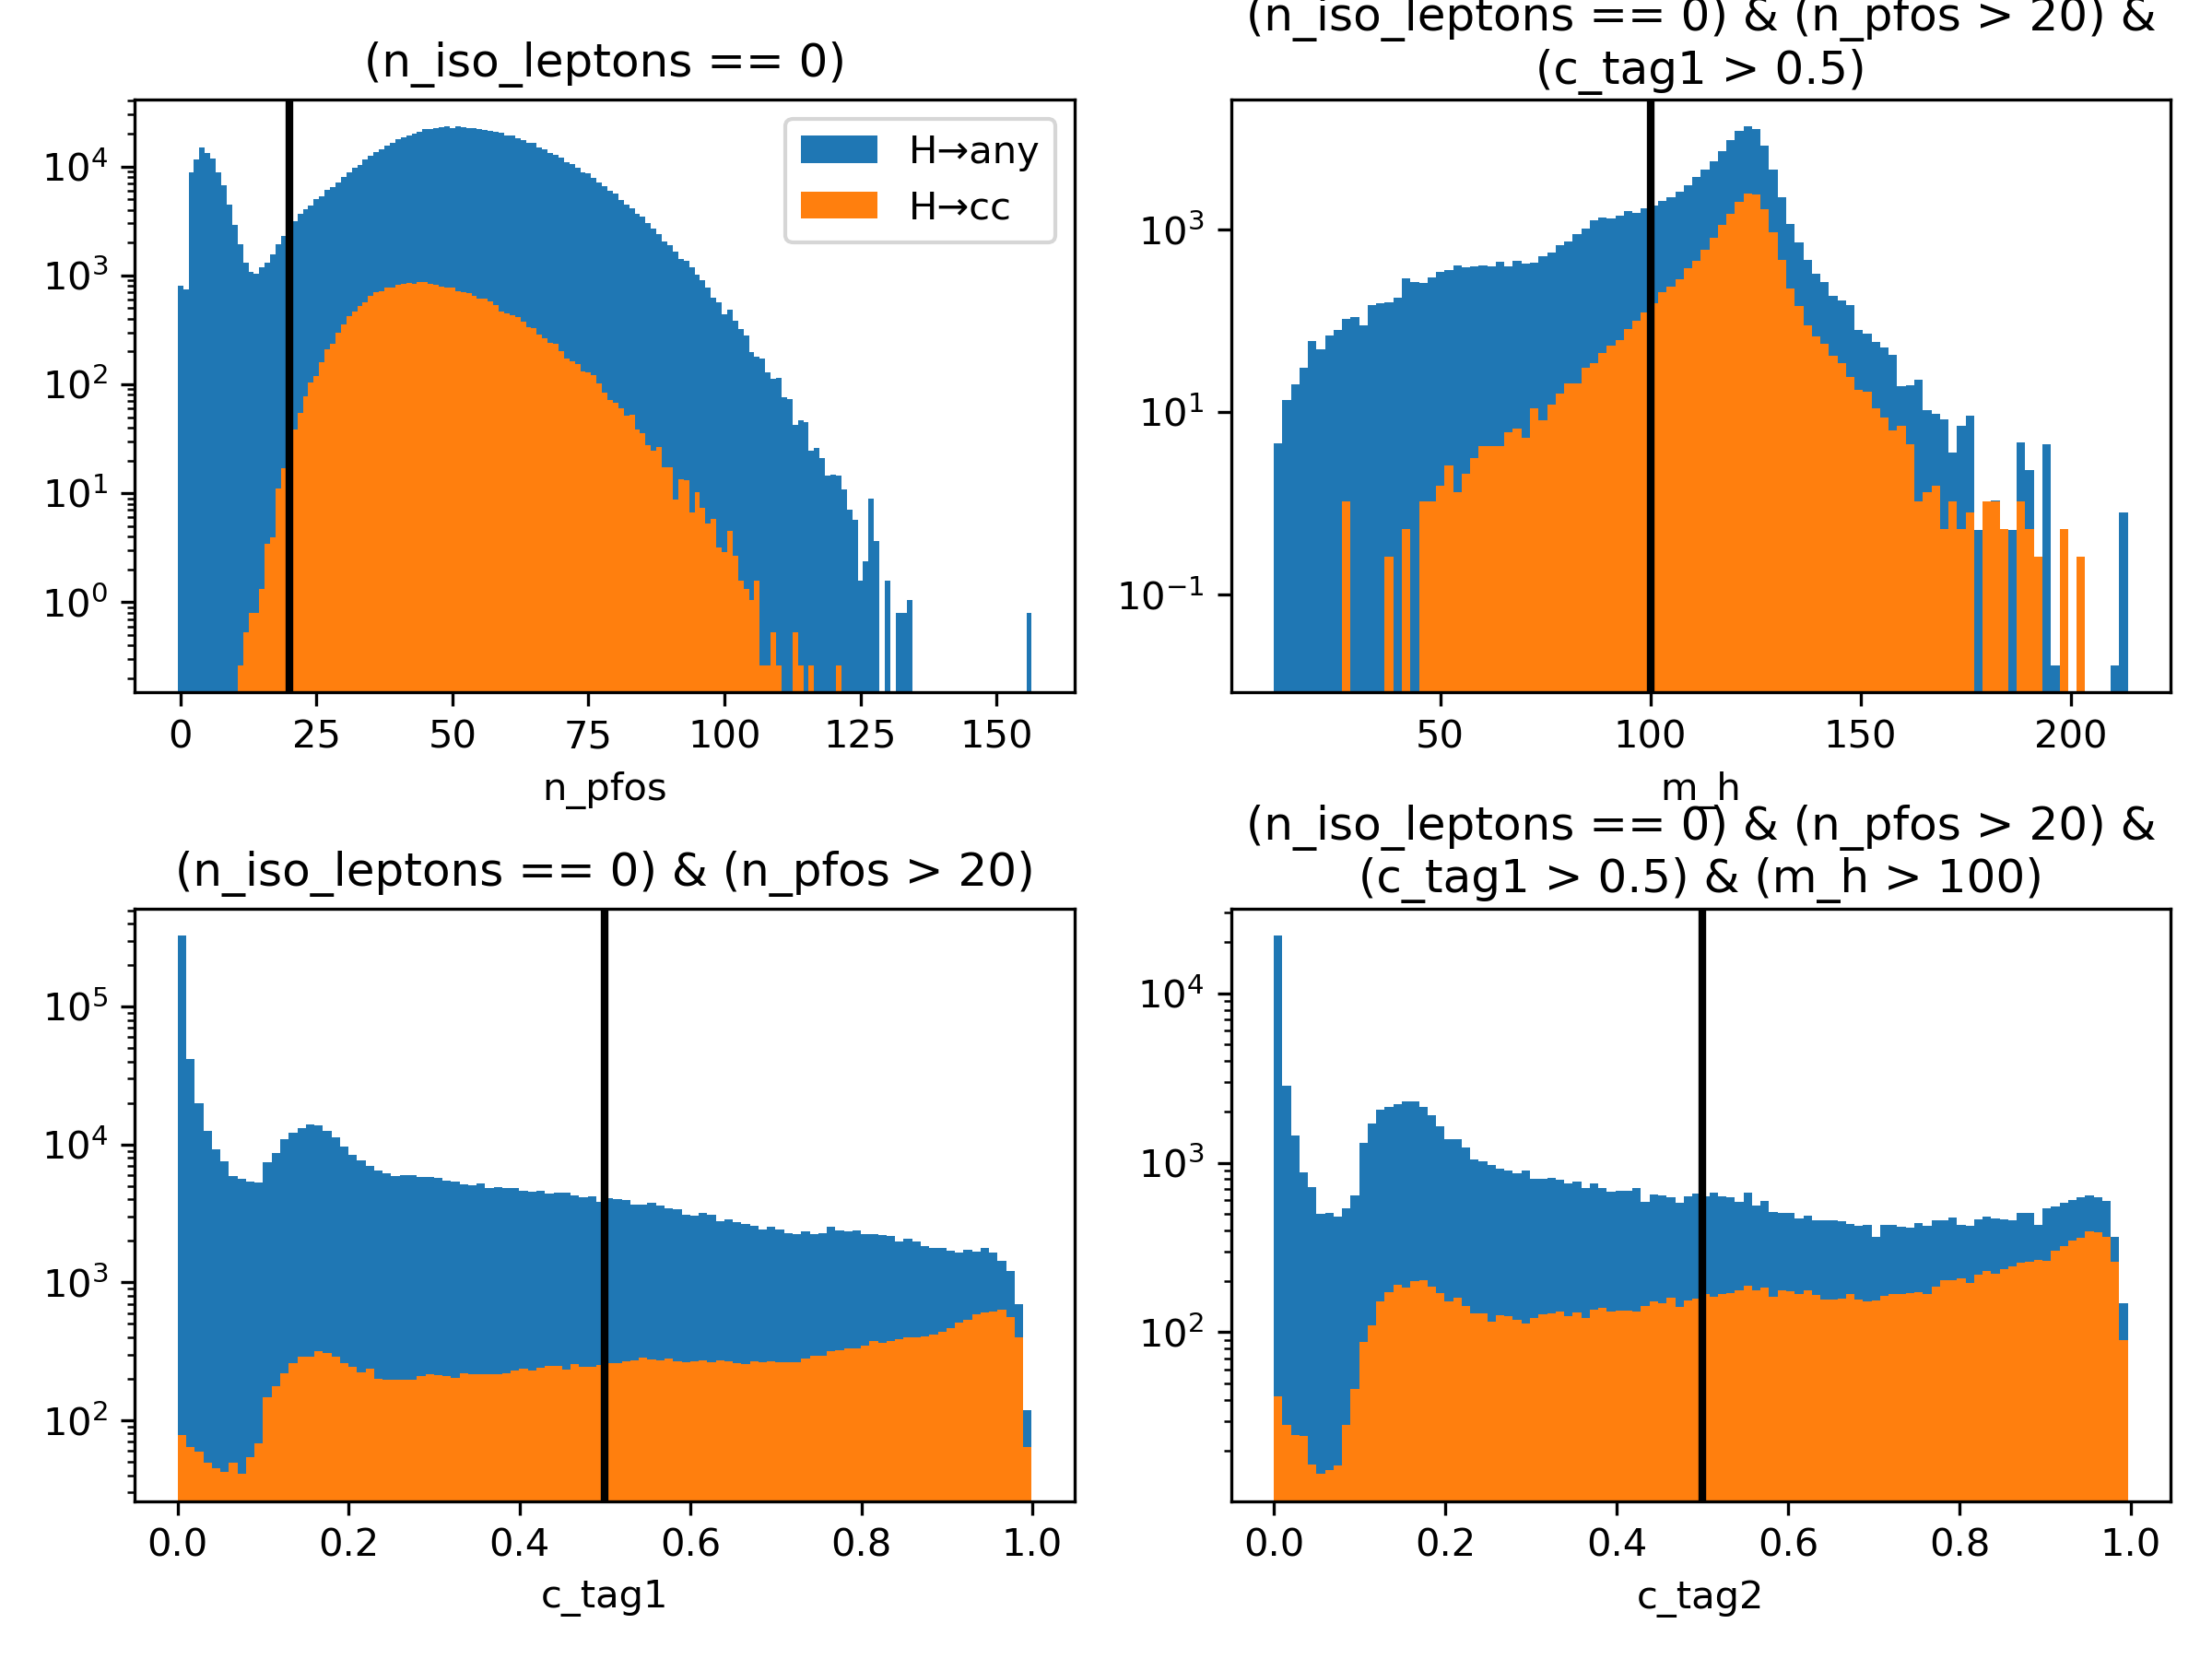
\includegraphics[height=0.9\textheight, width=0.95\textwidth, keepaspectratio]
      {plot_factory/cc_category_build_up}
  \end{column}
  \end{columns}
\end{frame}

\begin{frame}{Categories}
    \begin{itemize}
        \item Reuse common tools:
        \begin{itemize}
            \item \texttt{LCFIPlus} for jet construction and flavor tagging.
            \item \texttt{IsolatedLeptonTaggingProcessor}, \texttt{IsolatedPhotonTaggingProcessor}.
        \end{itemize}
        \item Custom variables motivated by specific channels:
        \begin{itemize}
            \item $M_{\mu^+\mu^-}$, $M_{\gamma\gamma}$.
            \item Recoil of the leading (Isolated) Photon against $(E=M_H, \vec{p}=0)$ at rest \\ ($\approx60-100~\GeV$ for $H\to Z\gamma$).
            \item ...
        \end{itemize}
        \item Only use so-far not categorized events in classes further down in the list.
    \end{itemize}
\end{frame}

\begin{frame}{Category matrix}
  This shows how events from a given BR distribute among categories. E.g. $H\to W^+W^-$.
  \begin{columns}[c, onlytextwidth]
  \begin{column}{0.31\textwidth}
  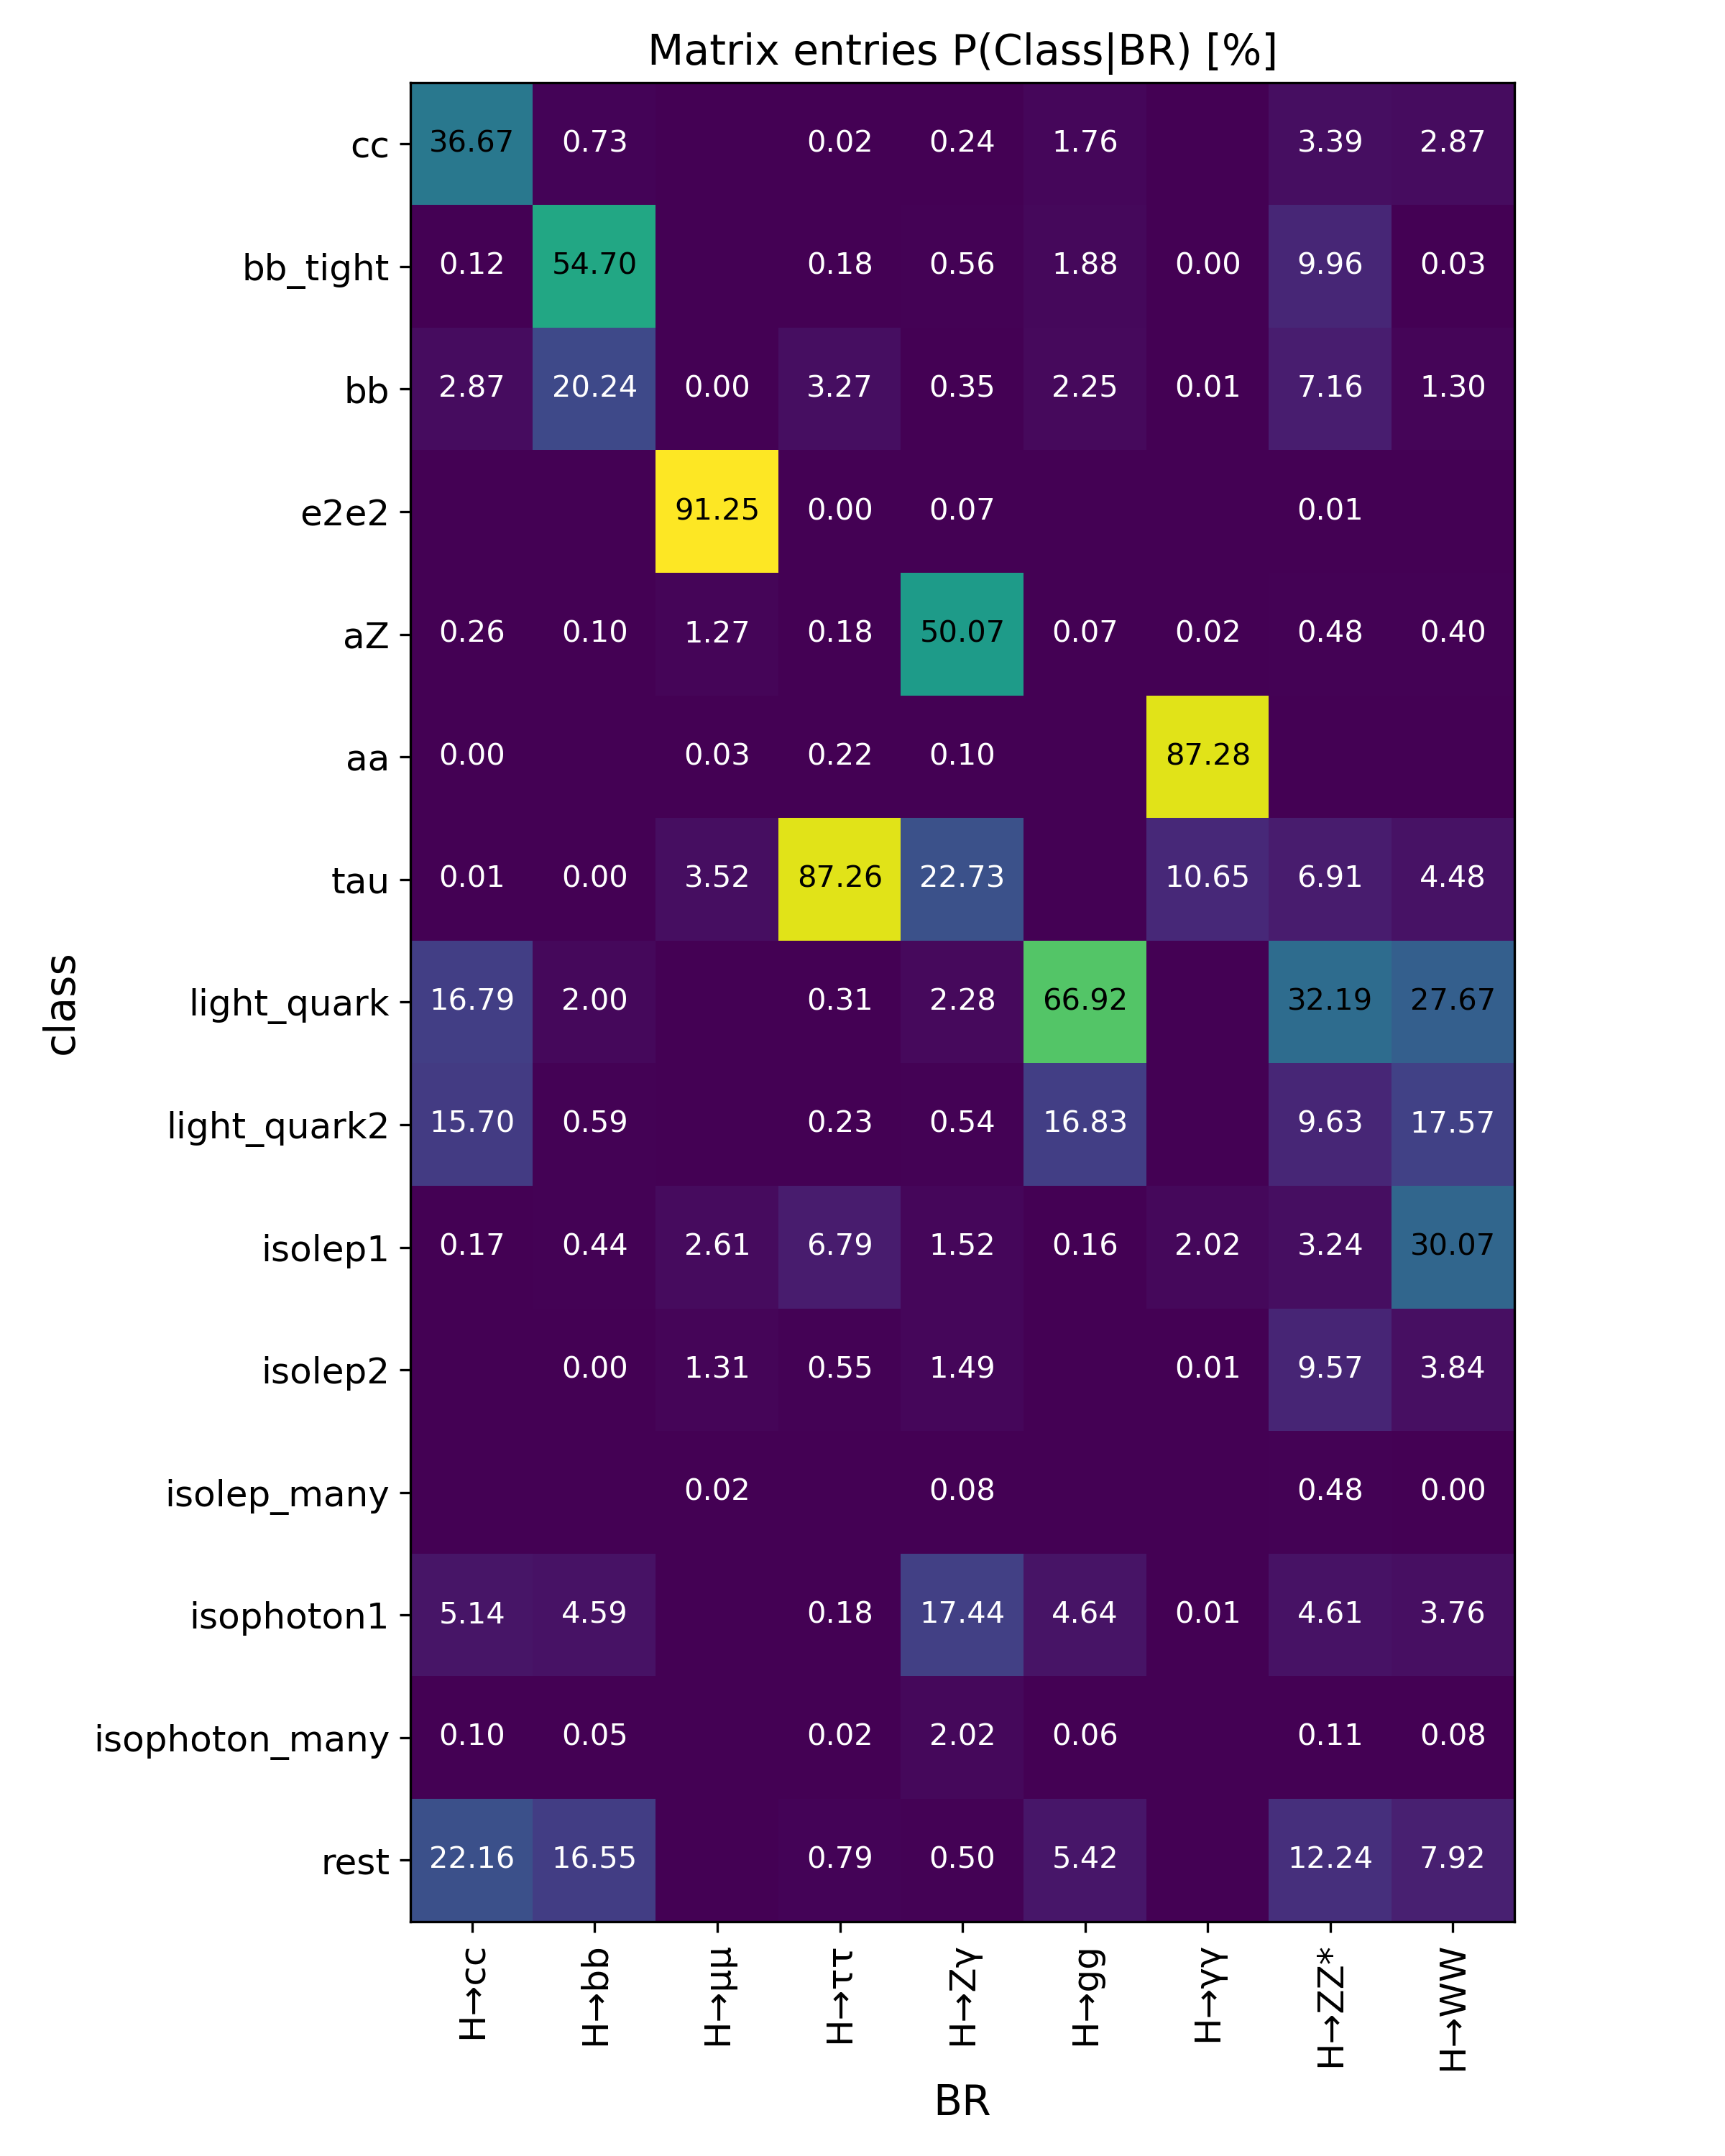
\includegraphics[width=0.95\textwidth, height=0.8\textheight, keepaspectratio]
      {plot_factory/overlay_free_probability_matrix}
  \end{column}
  \begin{column}{0.33\textwidth}
  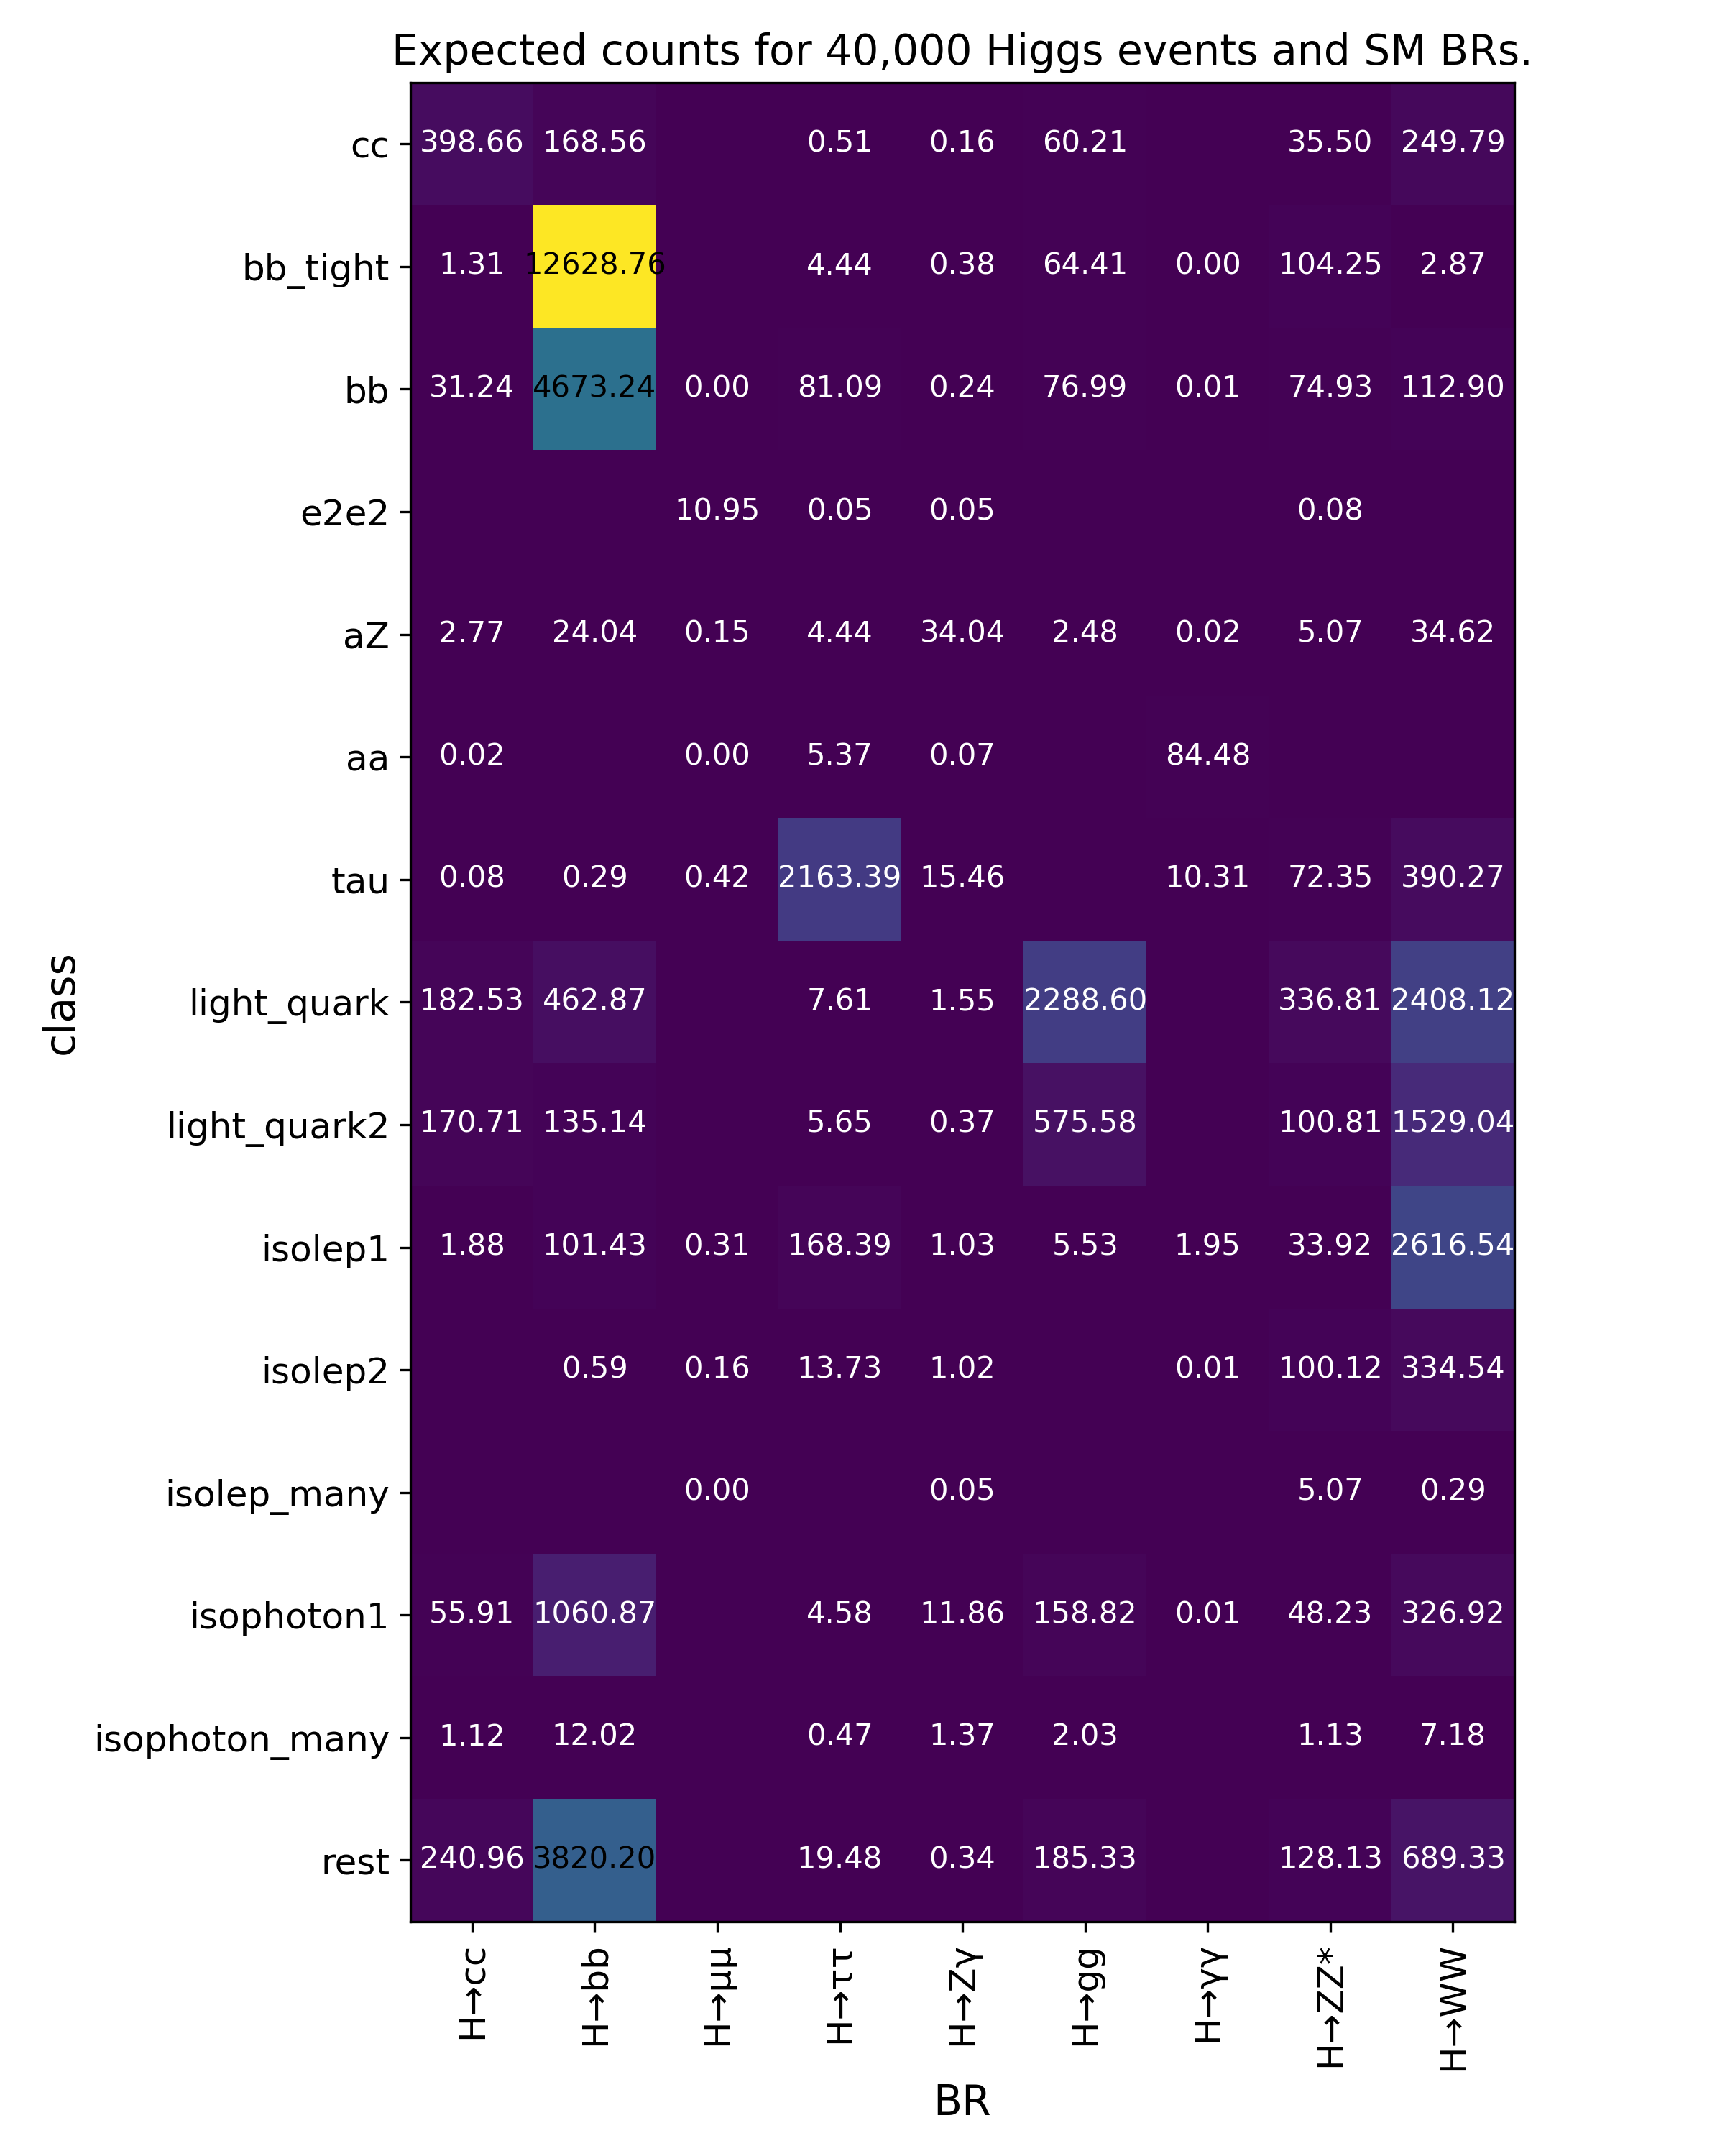
\includegraphics[width=0.95\textwidth, height=0.8\textheight, keepaspectratio]
      {plot_factory/overlay_free_expected_counts}
  \end{column}
  \begin{column}{0.35\textwidth}
        \hspace{0.5cm}
        \begin{minipage}[ht!]{0.45\linewidth}
            \centering
            % \resizebox{120pt}{180pt}{%
            \resizebox{120pt}{!}{\InputTex{extras/HWW_tikz.tex}}
        \end{minipage}
  \end{column}
  \end{columns}
\end{frame}